%% This is an example first chapter.  You should put chapter/appendix that you
%% write into a separate file, and add a line \include{yourfilename} to
%% main.tex, where `yourfilename.tex' is the name of the chapter/appendix file.
%% You can process specific files by typing their names in at the 
%% \files=
%% prompt when you run the file main.tex through LaTeX.
\chapter{Proposed Framework}\label{chap:framework}
\section{Proposed framework: tracking by detection}
\begin{figure}[htbp]
	\centerline{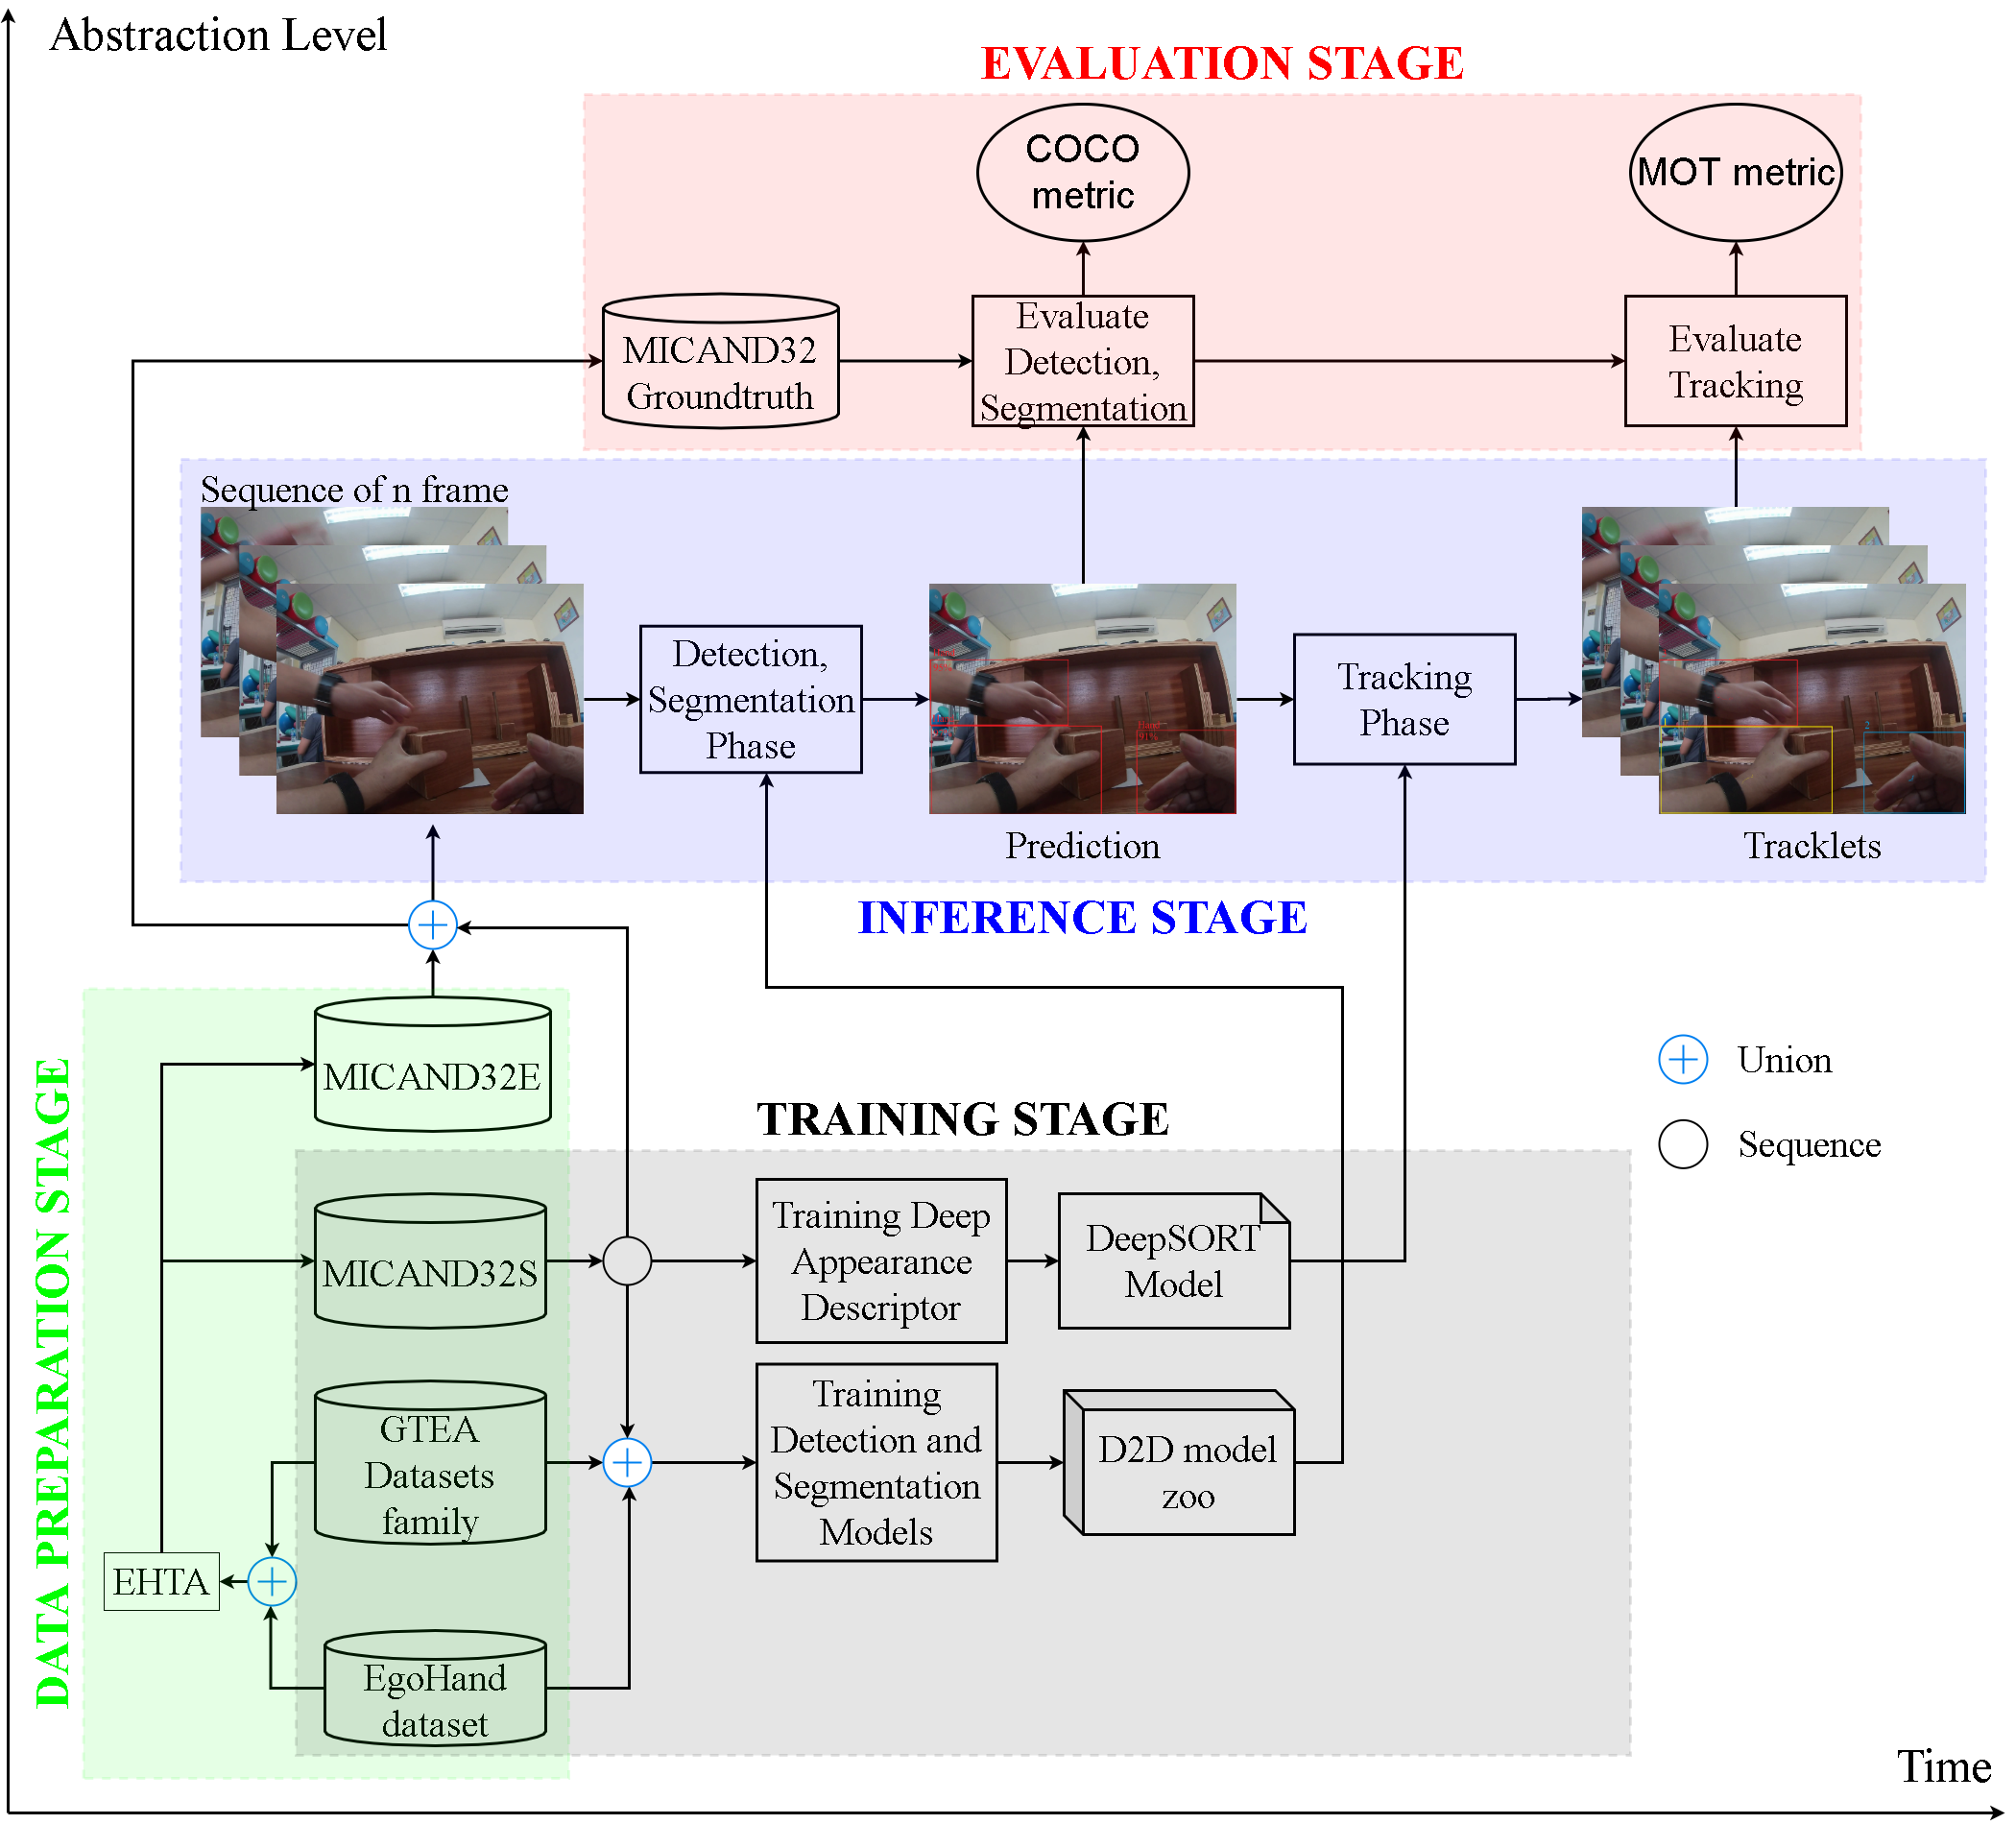
\includegraphics[width=1\linewidth]{Figs/proposedFramework.png}}
	\caption{Overview of proposed framework: D2D. The x-axis represents the time flow of the 4 stages. The y-axis regards the increasing degree of abstraction level of the stages.}
	\label{fig:framework}
\end{figure}
The framework proposed in this thesis consists of 4 stages: \begin{enumerate*}
	\item data preparation stage,
	\item training stage,
	\item inference stage,
	\item evaluation stage
\end{enumerate*}. Initializing with data preparation stage, the GTEA family and EgoHands datasets is collected and is pre-processed in order to keep only suitable and related ground-truth samples. These 2 datasets are used to construct EHTA model zoo by training hand detection and segmentation models from the first-person view. The annotators use semi-automatic EHTA tool to create the new dataset Micand32 descripted in chapter \ref{chap:method}, sub-section \ref{subsec:micand32}. Next is the models training stage. Three datasets including Micand32S, GTEA family and EgoHands datasets is used as fuel to train the hand detection and segmentation from egocentric vision, family of RCNN models and family of YOLO models. At the same time, a deep appearance descriptor is trained on distinct hand groups ground-truth in Micand32S. While the original DeepSORT's descriptor is made in people tracking context, the descriptor trained in the thesis is made well suited for deep metric learning in this egocentric hand context. Detail training techniques are reported in section \ref{sec:trainingstage}. Following the training stage is the inference stage in which all the videos in Micand32 datasets is tested. For each sequence of n frames, each frame in turn is fed respectively into the detection and segmentation phase to get the prediction which locate the hand’s bounding boxes, masks and their confidence scores. This phase requires user to select detection or segmentation algorithm from pre-trained D2D model zoo. Frames with detections are then fed into tracking phase. This phase also requires user to choose tracking algorithm SORT or DeepSORT. The tracking phase indicates the identifications of egocentric hands with their trajectories in the whole video. Section \ref{sec:inferstage} explains in detail the inference procedure. Finally, the evaluation stage encounters. Detection bounding boxes and segmentation masks is be evaluated by comparing with Micand32’s ground-truth. This result is measured in COCO format. The hand’s tracklets is evaluated and reported in MOT Challenge format. Detail evaluation criteria is described in section \ref{sec:evacri}. 
\section{Training stage} \label{sec:trainingstage}
\begin{figure}[htbp]
	\centerline{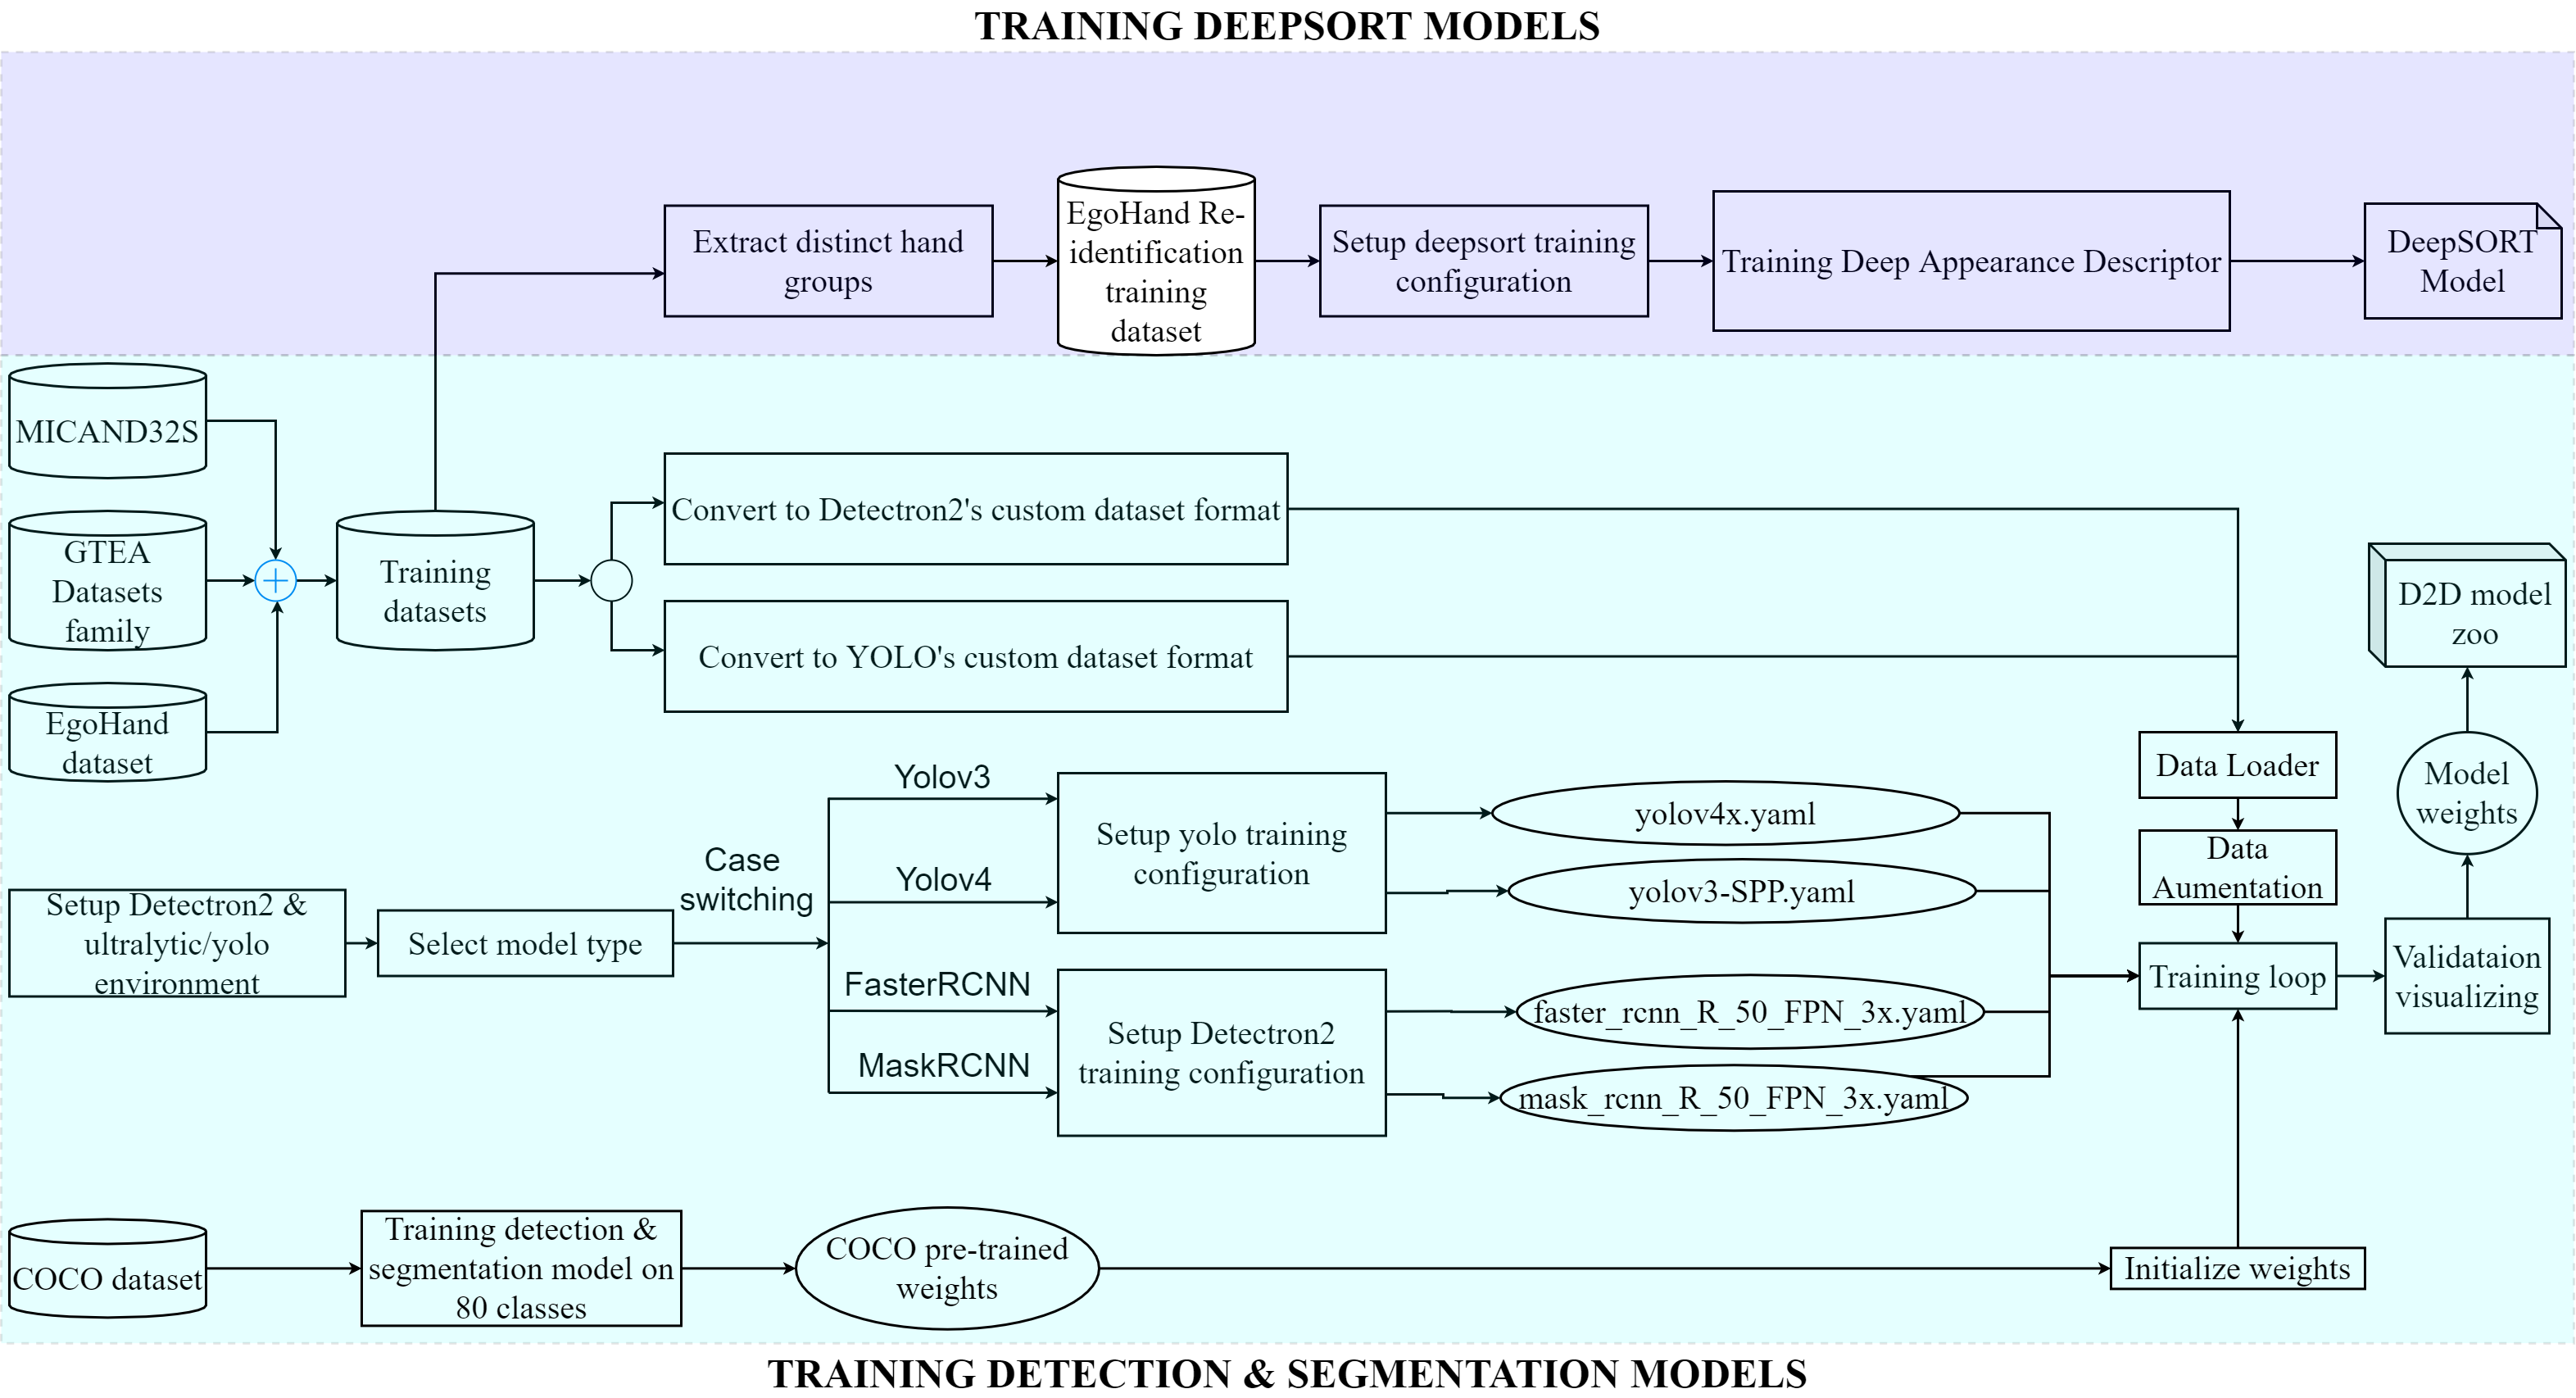
\includegraphics[width=1\linewidth]{Figs/trainingStage.png}}
	\caption{Workflow of the training stage.}
	\label{fig:trainingstage}
\end{figure}
The training stage shown in Figure \ref{fig:trainingstage} consist of parts: \begin{enumerate*}
	\item training detection and segmentation models,
	\item training DeepSORT model
\end{enumerate*}. Input of both parts are the combination of 3 datasets: Miand32S, GTEA family and EgoHands dataset. The first part will generate D2D model zoo which consists 4 types of models, 2 from yolo family and 2 from RCNN family. The second part trains a CNN for deep appearance descriptor for cosine metric learning \cite{DBLP:journals/corr/abs-1812-00442} in DeepSORT. Detail implementation is explained as follow.
\subsection{Training detection and segmentation models}
Initially I setup programming environment which consists 2 frameworks: Detectron2 \cite{wu2019detectron2} for RCNN model family and Ultralytics \cite{ultralytics} for YOLO model family.
Detectron2 is a complete rewrite of the previous version Detectron, and it originates from maskrcnn-benchmark. The platform is now implemented in and powered by the PyTorch deep learning framework. Through a new modular design, Detronron2 is flexible and scalable, and can provide fast training on a single or multiple GPU servers. Detectron2 includes high-quality implementations of state-of-the-art object detection algorithms, including DensePose, panoptic feature pyramid networks, and numerous variants of the pioneering Mask R-CNN model family also developed by FAIR. Its scalable design makes it easy to implement cutting-edge research projects without having to spend the entire code base. The requirements of installing Detectron2 includes: Linux with Python 3.6+, Pytorch 1.4+ and torchvision that matches the PyTorch installation, OpenCV need by demo and visualization. In this thesis, I build Detectron2 from source. The compilers gcc and g++ version 5+ are required, and ninja is recommended for faster build. After having these prerequisites, I clone the Detectron2 repositories and install it via pip from the local clone.
The Ultralytics open-source research into future object detection methods is represented via this repository \cite{ultralytics}. The requirements of install Ultralytics is Python 3.8 or later with all dependencies includes Cython, matplotlib, numpy, OpenCV, pillow, PyYAML, scipy, tensorboard, tqdm, pycocotools, scikit-learn, seaborn, coremltools and onnx. I build Ultralytics from source by cloning their github repository and install via pip.
After installing programming environments, users have to select the model type to train. There are 4 main models integrated in this thesis's framework, the RCNN family consists FasterRCNN and MaskRCNN, while the YOLO family consists Yolov3 and Yolov4. Depending on case of model selection, D2D switches to appropriate branch of setting up training configurations. For the RCNN family, Detectron2 supports different backbone network architectures such as ResNET \{50, 101, 152 \}|, FPN, VGG16, etc. In this thesis, I choose the standard configs, FasterRCNN\_R\_50\_FPN\_3x and MaskRCNN\_R\_50\_FPN\_3x with backbone Resnet 50 layers, feature pyramid network 3x architecture. The config file is saved in a ".yaml" format file. Table \ref{tab:fastConfig} represents a typical configuration for FasterRCNN\_R\_50\_FPN\_3x.
For the YOLO family, Ultralytics supports different model checkpoints type, and in this thesis, I choose the standard YOLOv3-SPP and YOLOv4x. Training configuration is also saved in a “.yaml” format file. Table \ref{tab:yoloConfig} represents a typical configuration for Yolov4x.
\\It should be noted that in this thesis the number of classes for training is 1 class “hand”. The initial weights is pre-trained on COCO dataset with 80 classes. The GTEA datasets family, EgoHands dataset and Micand32S datasets is repored in chapter \ref{chap:method}, section \ref{subsec:micand32}, all of them are merged into 1 training dataset. To let detectron2 know how to obtain a custom dataset, I implement a function that returns the items in training datasets. The standard representation for a dataset is combination of multiple dictionaries, each dictionary contains information about one image. The dictionary may have the following fields as in \ref{tab:d2custom}.
Ultralytics also requires exporting custom dataset labels to YOLO format, with one “*.txt” file per image. The “*.txt” file specifications are: (1) one row per object; (2) each row is “class x\_center y\_center width height” format; (3) box coordinates must be in normalized xywh format (from 0 - 1). If boxes are in pixels, divide x\_center and width by image width, and y\_center and height by image height; (4) class numbers are zero-indexed. Each image's label file should be locatable by simply replacing “/images/*.jpg” with “/labels/*.txt” in its pathname.

Data loader is the component that provides data to models. A dataloader usually takes raw information from datasets, and process them into a format needed by the model in training loop. Augmentation is an important part of training. Detectron2’s data augmentation system aims at addressing the following goals: (1) allow augmenting multiple data types together (e.g., images together with their bounding boxes and masks); (2) allow applying a sequence of statically-declared augmentation. For Ultralytics, a Mosaic Dataloader is used for training. The data augmentations used are horizontal and vertical flip, resize, Gauss noise, random brightness contract, crop, median blur, color distortion, gamma, converting color space; some of them are illustrated in Figure \ref{fig:augmentation}.
\begin{figure}[!htb]
	\centerline{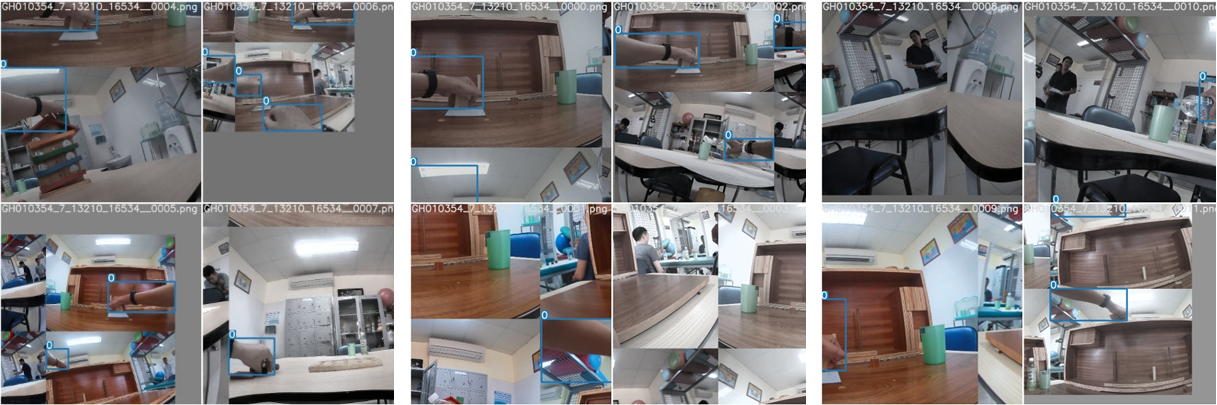
\includegraphics[width=1\linewidth]{Figs/augmentation.png}}
	\caption{Pictorial of data augmentations.}
	\label{fig:augmentation}
\end{figure}
With the benefits of transfer learning techniques discussed in \cite{DBLP:journals/corr/abs-1808-01974}, in this thesis, I start from the pre-trained weights on 80 classes in COCO datasets and fine-tune it for the particular “hand” classes. Training loop runs with defined configurations and augmented data. Training time for Yolov3, Yolov4, FasterRCNN and MaskRCNN in this thesis are respectively 36, 40, 46 and 50 hours.
The visualization of training steps is available via Tensorboard during training time as in \ref{fig:tensorboard}.
\begin{figure}
	\centerline{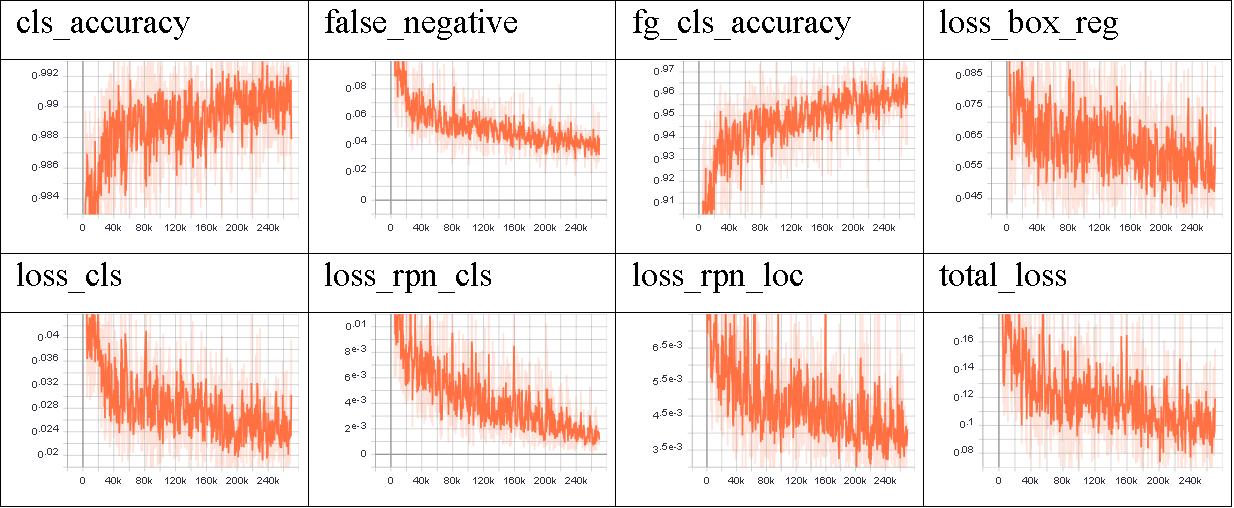
\includegraphics[width=1\linewidth]{Figs/tensorboard.png}}
	\caption{FasterRCNN\_R\_50\_FPN\_3x losses visualization during training time.}
	\label{fig:tensorboard}
\end{figure}
After training, the framework generates the D2D model zoo which contains 4 model with corresponding weights save in “.h” data format and will be used in the inference stage.
\subsection{Training deep appearance descriptor for DeepSORT} \label{subsec:train_deep}
The original DeepSORT is used for person tracking task – a familiar issue in which a given query image is used to look at a huge gallery of images that have been gathered at distinct moments, lighting environments, actions performing that may contain the same individual. To customize it on egocentric hand tracking mission, it firstly requires an egocentric hand re-identification dataset to train the appropriate appearance descriptor. As the best of my knowledge, there are very few public egocentric hand re-identification datasets available \cite{9064606}. From the analysis of 3 datasets described in chapter \ref{chap:method}, section \ref{sec:datasets}, I build a new egocentric hand re-identification dataset from the identity information annotations. Images of hands are extracted and cropped from these 3 datasets using the bounding box information and also resized to the same size (100, 100) as recommendation in  \cite{DBLP:journals/corr/abs-1812-00442}. As a result, there are in total 40 identities (26 subject from GTEA + 4 subject from EgoHands + 10 subject from Micand32S = 40 subjects) and 29324 images in this egocentric hand re-identification dataset. The sample of the images used in this dataset is shown in \ref{fig:reid}.
\begin{figure}[!htb]
	\centerline{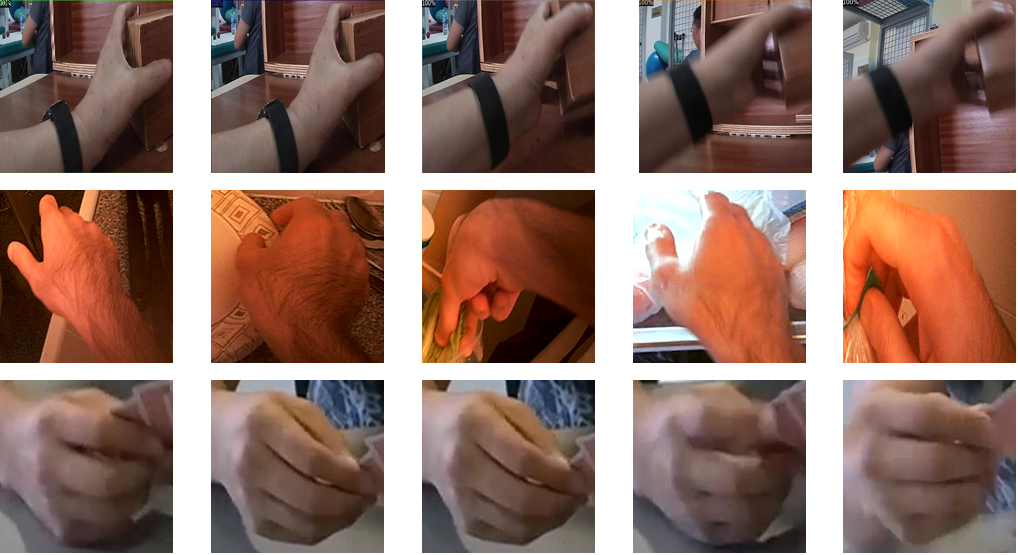
\includegraphics[width=1\linewidth]{Figs/reid.png}}
	\caption{Images from the self-generated egocentric hand re-identification dataset. Images in the same row has the same identity.}
	\label{fig:reid}
\end{figure}
Having obtained the egocentric hand re-identification dataset, I train the CNN to get the appearance descriptor. The train and test sets were slit into 80\% and 20\% respectively and both were structed by place all the images of one identity into a specific numbered folder for both train and test sets. I setup the training configuration as in Figure \ref{fig:descriptor}. The programming environment in which the training process performed is python 3 with PyTorch framework, numpy, scipy, sklearn, pillow, vizer and edict package.
The training chart obtained is shown in \ref{fig:descriptor}. It tooks 40 hours to train this CNN.
\begin{figure}[!htb]
	\centering
	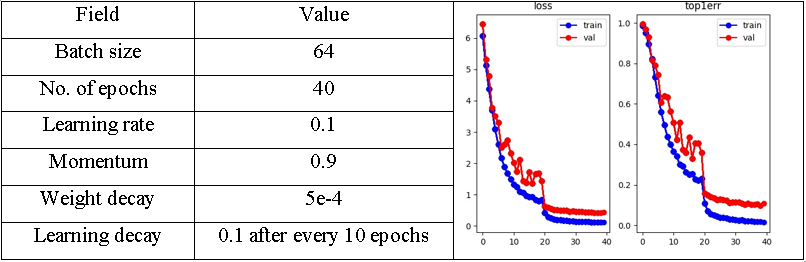
\includegraphics[width=\linewidth]{Figs/training_descriptor.png}
	\caption{Left: training configuration of DeepSORT’s appearance descriptor. Right curve of total loss and top1-error during training loop.}
	\label{fig:descriptor}
\end{figure}
\section{Inference stage}\label{sec:inferstage}
\begin{figure}[htbp]
	\centerline{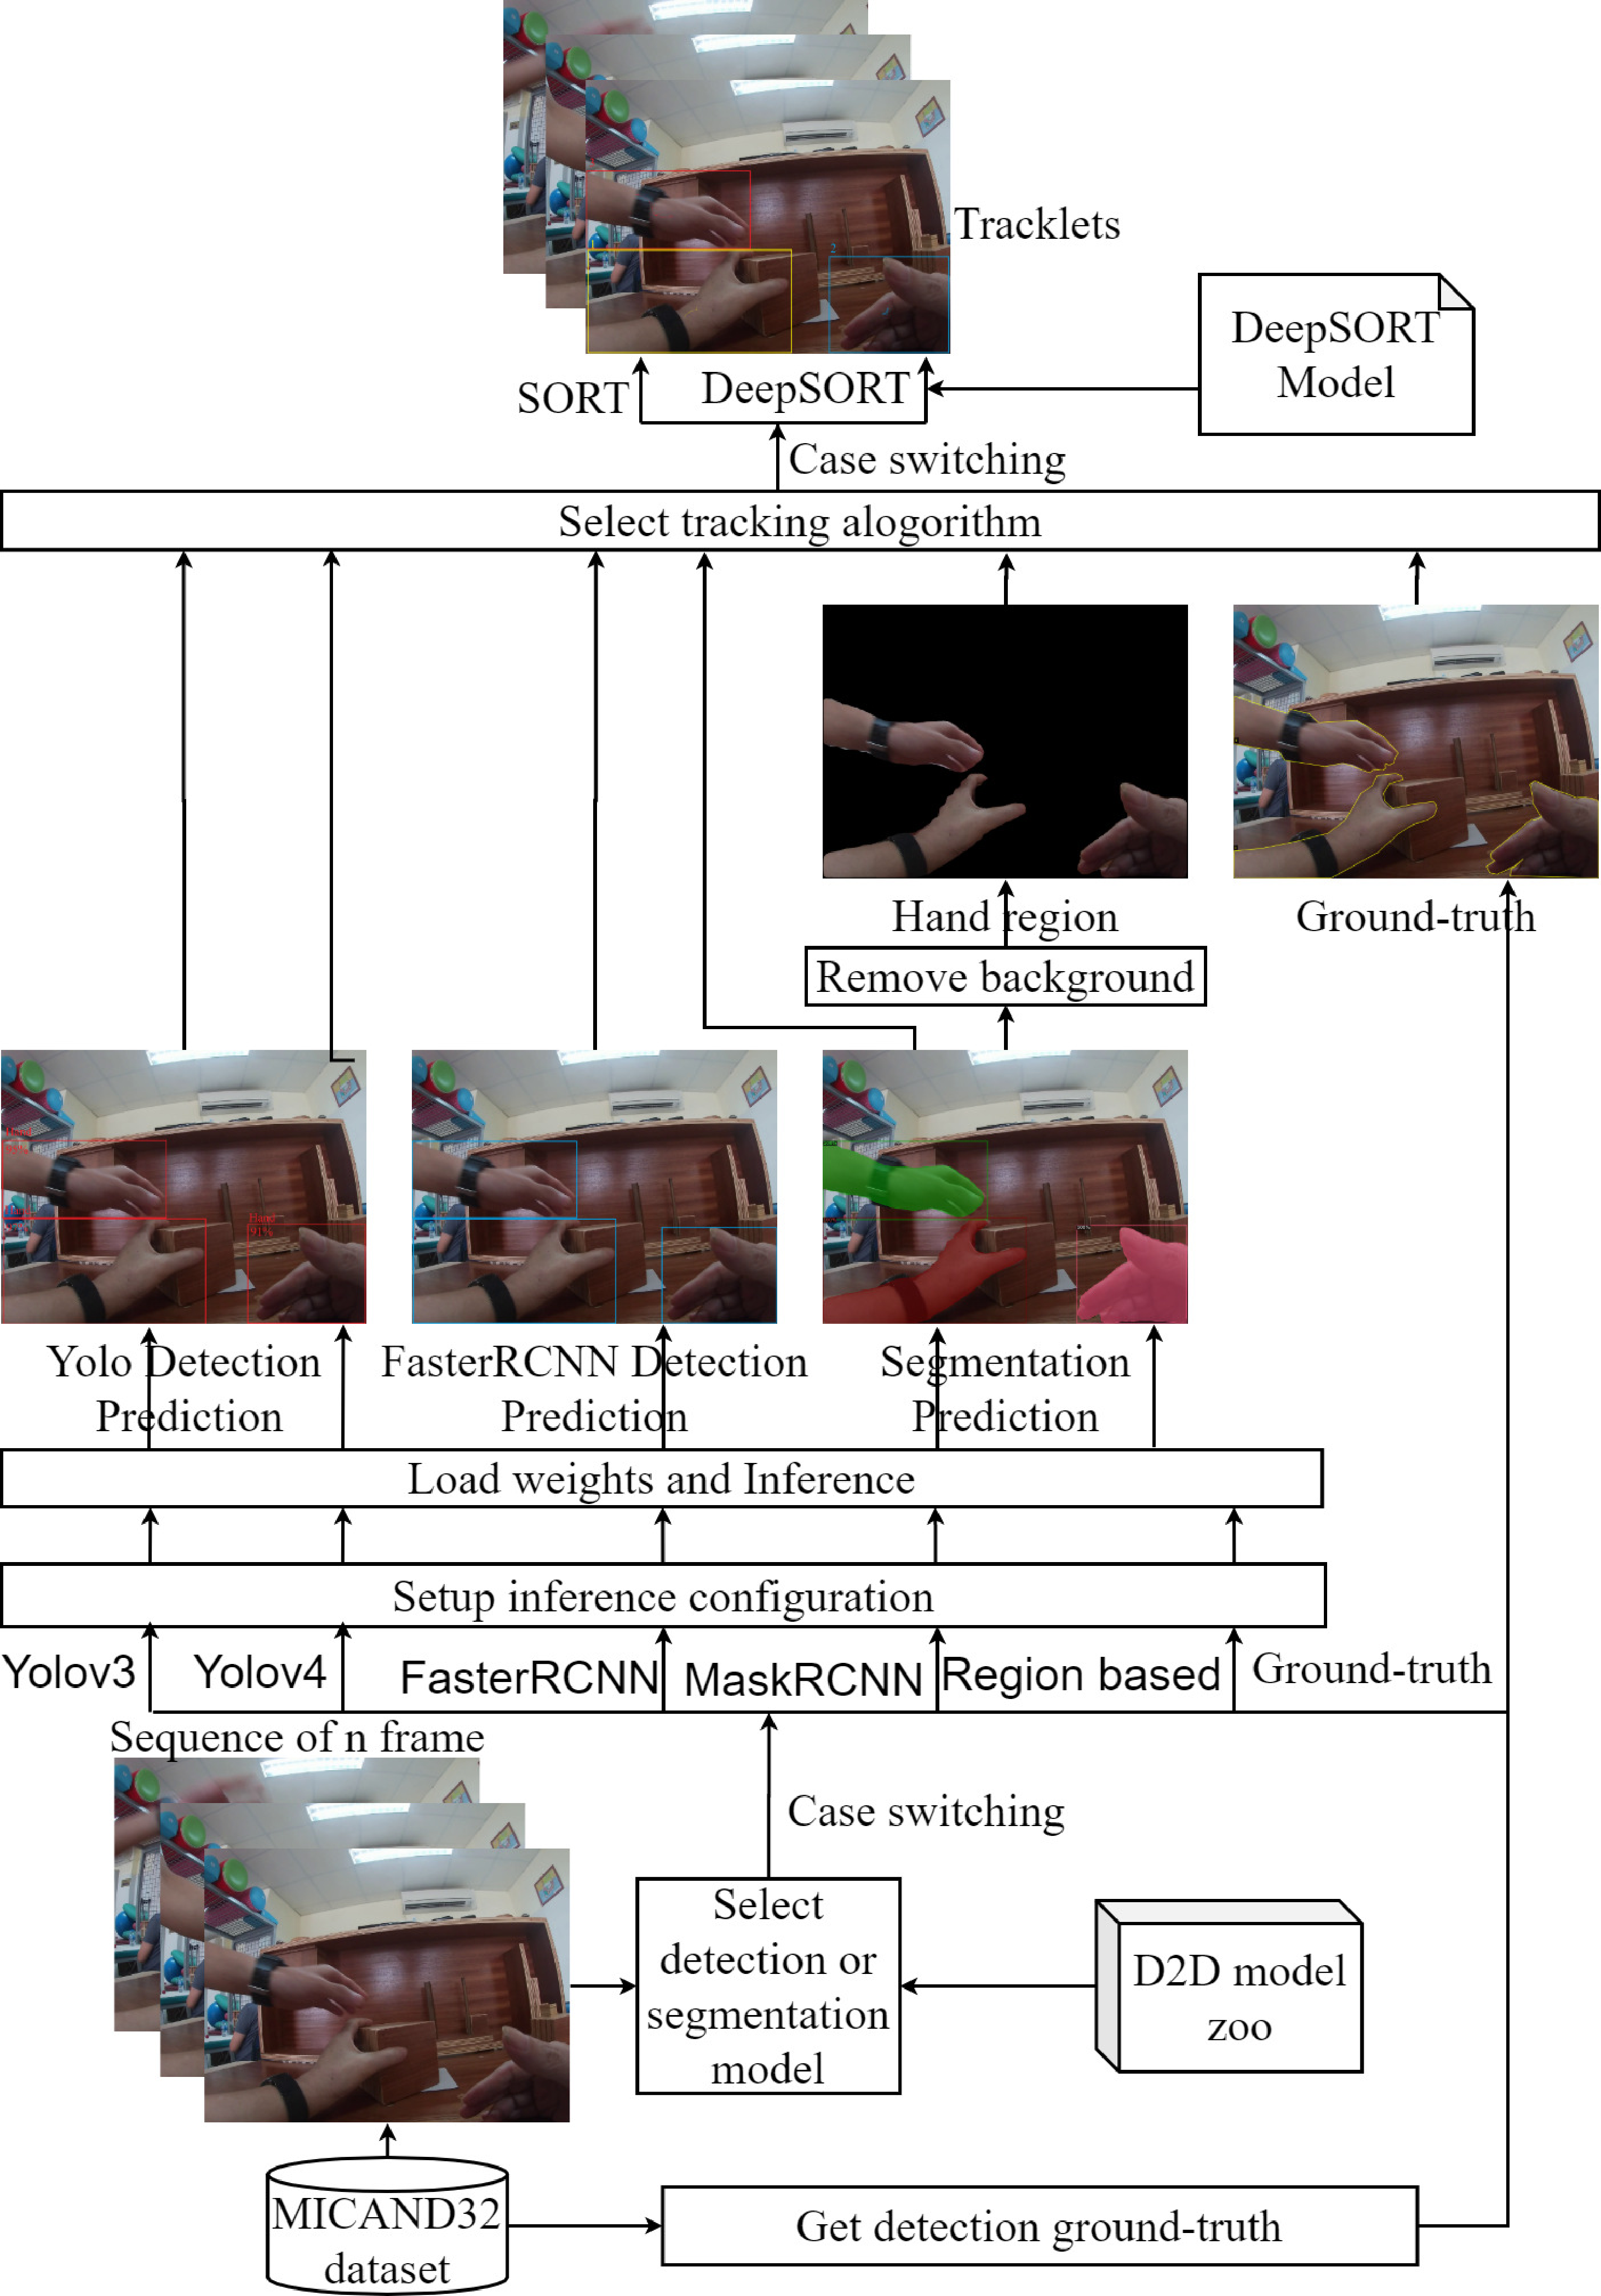
\includegraphics[width=\textwidth]{Figs/inferenceStage.eps}}
	\caption{Workflow of inference stage.}
	\label{fig:inferenceStage}
\end{figure}
In inference stage \ref{fig:inferenceStage}, each of 32 videos from Micand32 dataset will be tested in turn. Initially Each frame is fed into the detection phase in chronological order. Next, users select a detection or segmentation model from the D2D model zoo which was already trained in training stage. In order to analyze the affection of the detection phase on tracking phase, the detection ground-truth of Micand32 is also available for user to select in this step. As a consequence, 6 options are available: Yolov3\_spp, Yolov4x, FasterRCNNR50FPN3x, MaskRCNNR50FPN3x, MaskRCNNR50FPN3x with region based and detection ground-truth. Depending on the chosen model type, the D2D framework will setup inference configurations. For example, the default confidence threshold in this thesis is 50\%. Appropriate pre-trained weights will be loaded from the D2D model zoo in “.h” format and the inference process will begin. For detection models which includes yolo model family and FasterRCNNR50FPN3x, each prediction on image is represented in the following format: \(pred^i = [x_0^i, y_0^i, x_1^i, y_1^i, c^i]\) where \(pred^i\) is the i-th prediction with \((x_0^i, y_0^i),  (x_1^i, y_1^i)\), is respectively the top-left and bottom-right vertex coordinate of the i-th bounding box and ci is the current confident score of this bounding box. For MaskRCNNR50FPN3x, each prediction will consist one more field: \(pred^i = [x_0^i, y_0^i, x_1^i, y_1^i, pol^i, c^i]\) where the \(pol^i\) is the polygon of the mask in RLE format. For MaskRCNNR50FPN3x with region-based option, after obtaining the mask predictions, the framework will execute background subtraction in order to keep only hand region. This is intended to make the deep appearance descriptor in DeepSORT focus more on the hand region. In the following step, users will select the tracking algorithm, include: SORT or DeepSORT. For SORT, detection will be processed in Kalman filter and then associated by the Hungarian algorithm as explained in chapter 2, section 2.3. For DeepSORT, the deep appearance descriptor will be loaded from the pre-trained CNN in the training stage. Tracklets for the whole sequences will be compared with the tracking ground-truth in evaluation stage in order to analyze the effective of the algorithms.
\section{Evaluation stage}
Detail evaluation criteria and measurement metrics is reported in chapter \ref{chap:exp}, section \ref{sec:evacri}. The evaluation stage includes 2 parts: (1) evaluate detection and segmentation results; (2) evaluate tracking results. For detection and segmentation result, this thesis adopts the evaluation API from Detectron2 repository and the py-cocotools package. For tracking result, performance is measured according to the framework presented in \cite{DBLP:journals/corr/MilanL0RS16}. The authors provide evaluation scripts for official development kit of MOT Challenge. MOT16 was chosen since it is a compilation of other many metrics developed in an attempt to standardize evaluation of multiple object tracking. This devkit requires Python 3.7+, Matlab R2020a, matlab python engine, pandas and pytz. Tracking result will be saved in simple comma-separated value (CSV) files. Each line represents one object instance and contains 9 values as show in Table \ref{tab:eva_cri_tracking}.
\begin{table}
	\centering
	\caption{Data format for both the inference result and ground-truth annotation of tracking.}
	\resizebox{\textwidth}{!}{%
		\begin{tabular}{|l|l|l|}
			\hline
			Position & Name                & Description                                                                                                                                                                                 \\ \hline
			1        & Frame number        & Indicate at which frame the object is present                                                                                                                                               \\ \hline
			2        & Identity number     & Each hand trajectory is identified by a unique ID                                                                                                                                           \\ \hline
			3        & Bounding box left   & Coordinate of the top-left corner of the pedestrian bounding box                                                                                                                            \\ \hline
			4        & Bounding box top    & Coordinate of the top-left corner of the pedestrian bounding box                                                                                                                            \\ \hline
			5        & Bounding box width  & Width in pixels of the hand bounding box                                                                                                                                                    \\ \hline
			6        & Bounding box height & Height in pixels of the hand bounding box                                                                                                                                                   \\ \hline
			7        & Confidence score    & It acts as a flag whether the entry is to be considered (1) or ignored (0)                                                                                                                  \\ \hline
			8        & Class               & Indicates   the type of object annotated. In this thesis, always (1)                                                                                                                        \\ \hline
			9        & Visibility          & \begin{tabular}[c]{@{}l@{}}Visibility   ratio, a number between 0 and 1 that says how much of the hand is visible.\\ Can be due to occlusion and due to image border cropping.\end{tabular} \\ \hline
		\end{tabular}%
	}
	\label{tab:eva_cri_tracking}
\end{table}
An example of such an annotation file is:
\begin{itemize}
	\item 1, 1, 1672, 763, 248, 245, 1, 1 ,1
	\item 1, 2, 1253, 426, 156, 200, 1, 1 ,1
	\item 2, 1, 1668, 774, 252, 234, 1, 1, 1
\end{itemize}
In this case, there are 2 hand in the first frame of the sequence, with identity tags 1, 2 and 1 hand in the second frame with identity tags 1.